\documentclass[11pt]{article}

\usepackage{amssymb, amsmath, lineno, enumitem, float, epstopdf, graphicx}
\usepackage{caption}
\usepackage{subcaption}
\usepackage[margin=0.75in]{geometry}
\title{Genealogical Properties under the Moran Model}\author{Arjun Biddanda}
\date{\today}
% Removes the page numbering
\pagenumbering{gobble}

\begin{document}
\maketitle
% \linenumbers

\section{Initial Derivations}

\subsection{Definitions and Notation}

There are many definitions for the Moran Model, but we will adopt the model according to the following definition:

\begin{enumerate}
	\item Choose one individual to ``die''
	\item Choose one individual (it may be the same individual) to reproduce and have 2 offspring
\end{enumerate}

Note that this differs considerably from the aspects of the Discrete-Time Wright-Fisher (DTWF) model in that by construction multiple-mergers are not allowed to occur within a generation. However, all of the other relevant genealogical properties are available for interrogation.

\subsection{Probability of Lineage Reduction}
Initially we want to derive the probability that the number of lineages is reduced from $n$ to $m$ from the $t^{\text{th}}$ to the $(t+1)^{\text{th}}$ generation :

\begin{equation*}
	p^{(t)}_{n,m} = 
	\begin{cases} 1 - \frac{n(n-1)}{N^2_{t+1}}  & \text{if $m = n$,}
		\\
		\frac{n(n-1)}{N^2_{t+1}} &\text{if $ m = n - 1$,}
		\\
		0 &\text{else.}
	\end{cases}
\end{equation*}

We note that as $t$ is increasing, we are moving farther back in time (e.g. the ($t+1)^{th}$ generation is gene generation immediately before the $t^{th}$. The rationale for the derivation is that in order to reduce the number of lineages by 1, we must pick one of $n$ individuals to then be ``replaced'' by one of $n-1$ individuals. 

This is a very simplistic representation of the Moran model and can be extended to support a higher birth rate (which can potentially yield multiple mergers). We plan to discuss these more general forms in greater detail towards the end of the analysis. 

We can then extend this to $p^{(t, t')}_{n,m}$, or the probability that $n$ samples in generation $t$ have $m$  ancestors in generation $t'$. Due to the construction of the Moran Model, we are required to bound the quantity $m$ such that $n-t' \leq m \leq n$, otherwise the probability is $0$. Thus we obtain the following recursion :

$$
\begin{aligned}
	p^{(t, t')}_{n,m} &= \Bigg[\frac{n(n-1)}{N_{t+1}}\Bigg] p^{(t, t'-1)}_{n-1, m} + \Bigg[1 - \frac{n(n-1)}{N_{t+1}}\Bigg] p^{(t, t'-1)}_{n,m}\\
	p^{(t, t)}_{n,n} &= 1\\
\end{aligned}
$$

The recursion holds when $t' \geq t$. Having this recursion relation allows us to look at lengths of time that are longer than just a single generation. This allows us to look at the long range time-scaling of the process that is needed to compare the Moran Model to the coalescent.  

We would expect that when the sample size gets larger, the proportion of lineages that are lost successively in the generations of the Moran model will be quite a bit higher. See Figure 1 for a direct comparison of the probability of $m$ descendents under the Moran Model with time scaled to equal the a generation in the DTWF model. 

\subsection{Expected Number of Lineages as a Function of Time (NLFT) under the Moran Model}

Now that we have the following we can think of time $t$ in much larger steps (e.g. in increments of $t_{scaled}$) such that we can now define the probability of having $m$ ancestral lineages (conditional on $n$ lineages at time $t = 0$. These results directly mirror those of Bhaskar et al, but now with the recursion derived for the Moran Model:

 \begin{equation*}
	 \mathbb{P}[A^M_n(t) = m] =
	 \begin{cases} 
		 \sum^n_{k=m}  p^{(t-t_{scaled}, t)}_{k,m} \mathbb{P}[A^M_n (t-t_{scaled}) = k],  &\text{if $t > 0$,}
	 	 \\
		 \delta_{n,m} &\text{if $t = 0$}
	 \end{cases}
 \end{equation*}

 Where $\delta$ takes a value of $1$ when $n=m$ and $0$ elsewhere. From this realization, we can directly calculate the NLFT in the Moran Model as:

 \begin{equation*}
	 \mathbb{E}[A^M_n(t)] = \sum^n_{m=1} m \mathbb{P}[A^M_n (t) = m]
 \end{equation*}

\subsection*{Expected Number of Lineages Under the Coalescent}

We use the moment-based method of Tavare [CITE] in order to compute the expectation and the variance of the NLFT (with no mutation) under the Kingman coalescent:

\begin{equation*}
	\mathbb{E}[A^C_n(t)] = \sum^n_{i=1} e^{-\binom{i}{2}\Omega(t)} (2i - 1) \frac{n_{(i)}}{n^{(i)}} 
\end{equation*}

\begin{equation*}
	Var[A^C_n(t)] = \sum^n_{i=1} e^{-\binom{i}{2}\Omega(t)}(2i-1)(i^2 - i + 1)\frac{n_{(i)}}{n^{(i)}} - \Bigg[\mathbb{E}[A^C_n(t)]\Bigg]^2
\end{equation*}

Where $n_{(i)}$ and $n^{(i)}$ are the falling and rising factorials respectively. Note that the $t$ measured here is in ``coalescent time'' and will need to be rescaled appropriately when considering the discrete generations that we have for our model. We can define the following function to denote the rescaling of time (following Bhaskar et al) :

\begin{equation*}
	\Omega(t) = \begin{cases}
		\int_{0}^t \frac{N_0}{N_\tau} d\tau &\text{under the DTWF}\\[2ex]
		\int_{0}^t \frac{N_0^2/2}{N_\tau^2/2} d\tau  &\text{under the Moran Model}
	\end{cases}
\end{equation*}

%\subsubsection{Sample Frequency Spectrum under the Moran Model}

%We would also like to obtain the expected Site Frequency Spectrum (SFS) under the Moran Model. We will use the same notation and general derivation as Bhaskar et al.

%We set the entry $\tau_{n,k}$ as the number of sites at which $k$ individuals carry the derived allele and $n-k$ individuals carry the ancestral allele. Thus we can then define the entire SFS as $\tau_n = (\tau_{n,1}, ..., \tau_{n,n-1})$. 

%We will further define $\gamma^{(t)}_{a,b}$ as a random variable representing the total branch length of a subtree that subtends a set of $a$ individuals in a larger set of $a+b$ individuals. 


\newpage

\subsection{Figures}

\begin{center}
	\begin{figure}[!ht]
		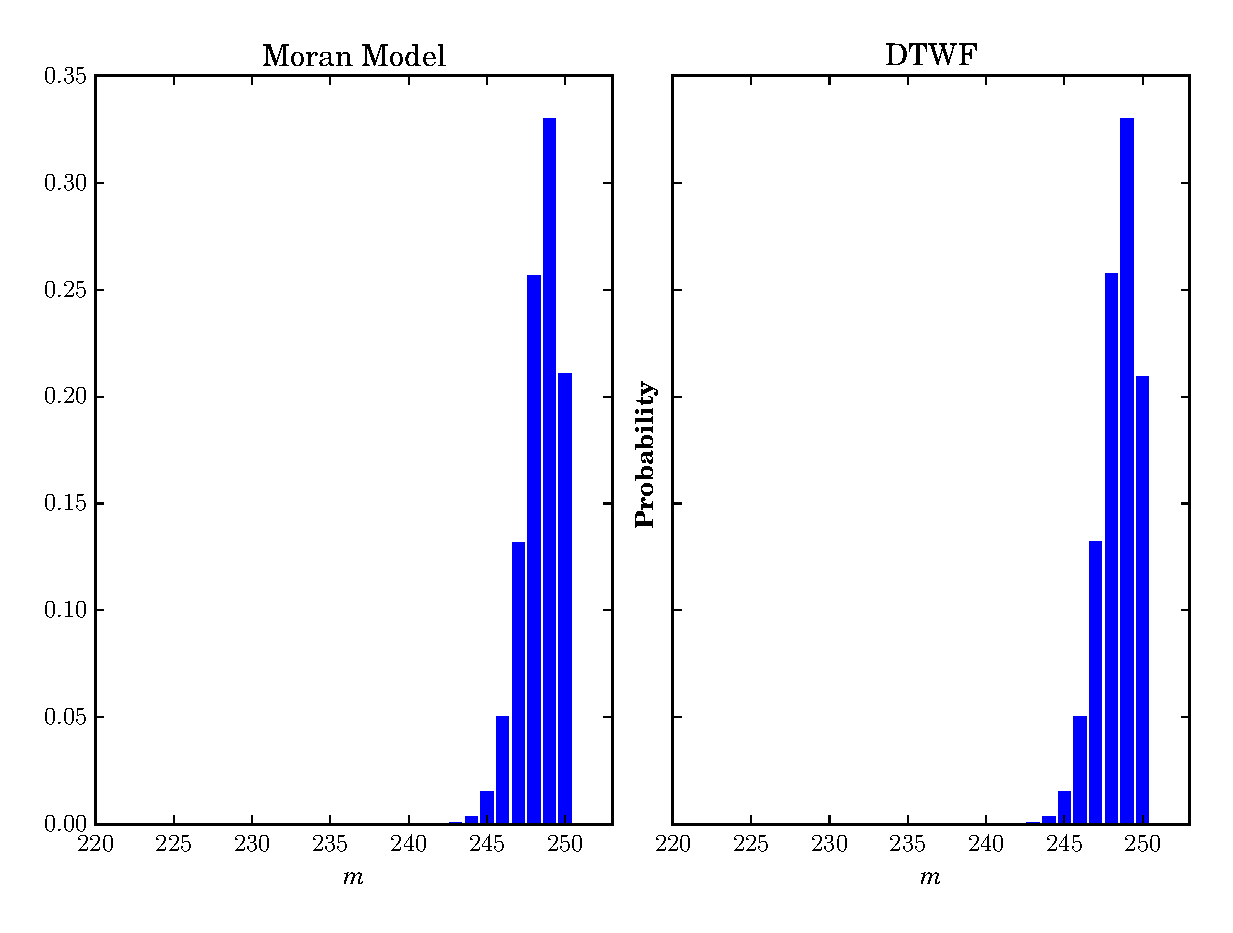
\includegraphics[scale=0.85]{../plots/moran_figure1}
		\caption{Comparing the distribution of parental lineages in the Moran Model and the Discrete-Time Wright-Fisher (DTWF) model. For both scenarios we maintained a constant population size of $N = 20000$ and a sample size of $n=250$. The results in the right pane correspond exactly to Supplementary Figure 2 in Bhaskar et al. We must note that in order to compare the Moran model to the DTWF we report the results after $N/2 = 20000/2 = 10000$ Moran generations in the left pane to equal a single DTWF generation. This scaling result is from Wakeley [CITE]. If we compare the expected number of ancestral lineages, $\mathbb{E}(m | Moran) = 247.45337685$ and  $\mathbb{E}(m | DTWF) = 247.45016269$}
	\end{figure}
\end{center}

\begin{center}
	\begin{figure}[!ht]
		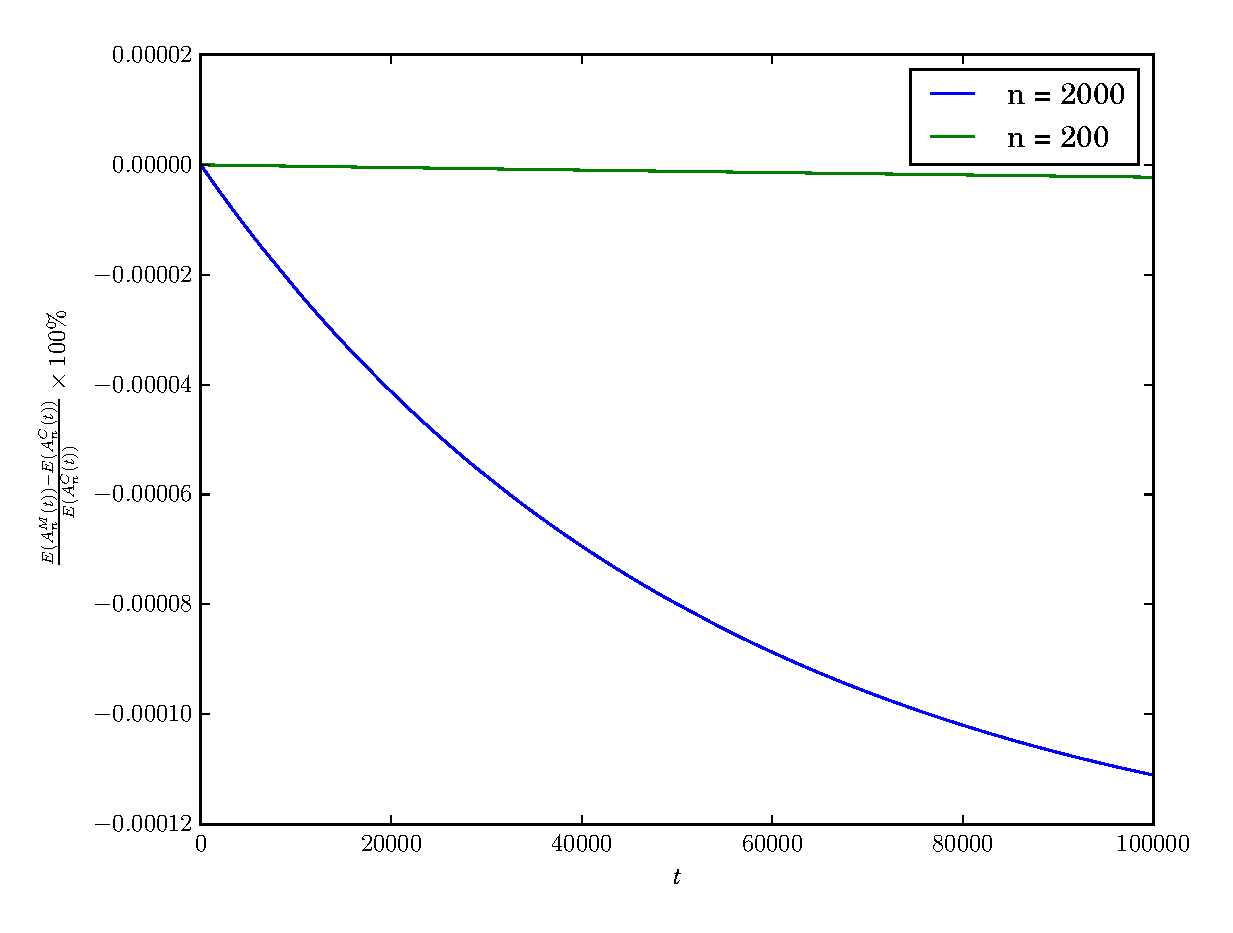
\includegraphics[scale=0.85]{../plots/moran_figure2}
		\caption{Comparing the distribution of parental lineages when the population size is relatively small ($N = 200$) with a sample size of $n=25$. We can see that under a smaller population size like this we can start to observe some differences in the ancestral DTWF model and the Moran model. Note that we have retained the same time scaling here as in the first figure as well.}
	\end{figure}
\end{center}

\begin{center}
	\begin{figure}[!ht]
		\begin{subfigure}[t]{\textwidth}
			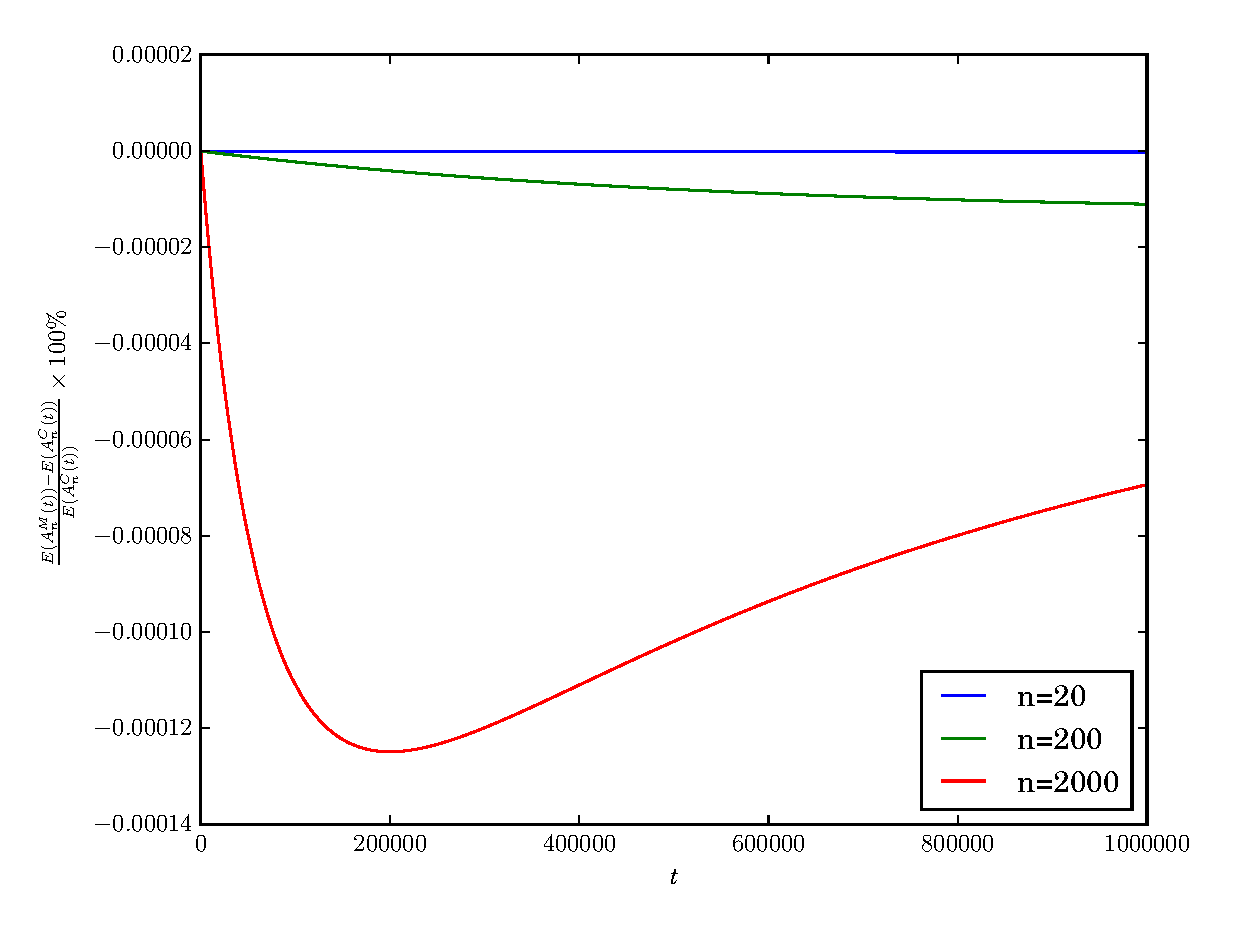
\includegraphics[scale=0.7]{../plots/moran_figure3}
		\end{subfigure}
		~
		\begin{subfigure}[t]{\textwidth}
			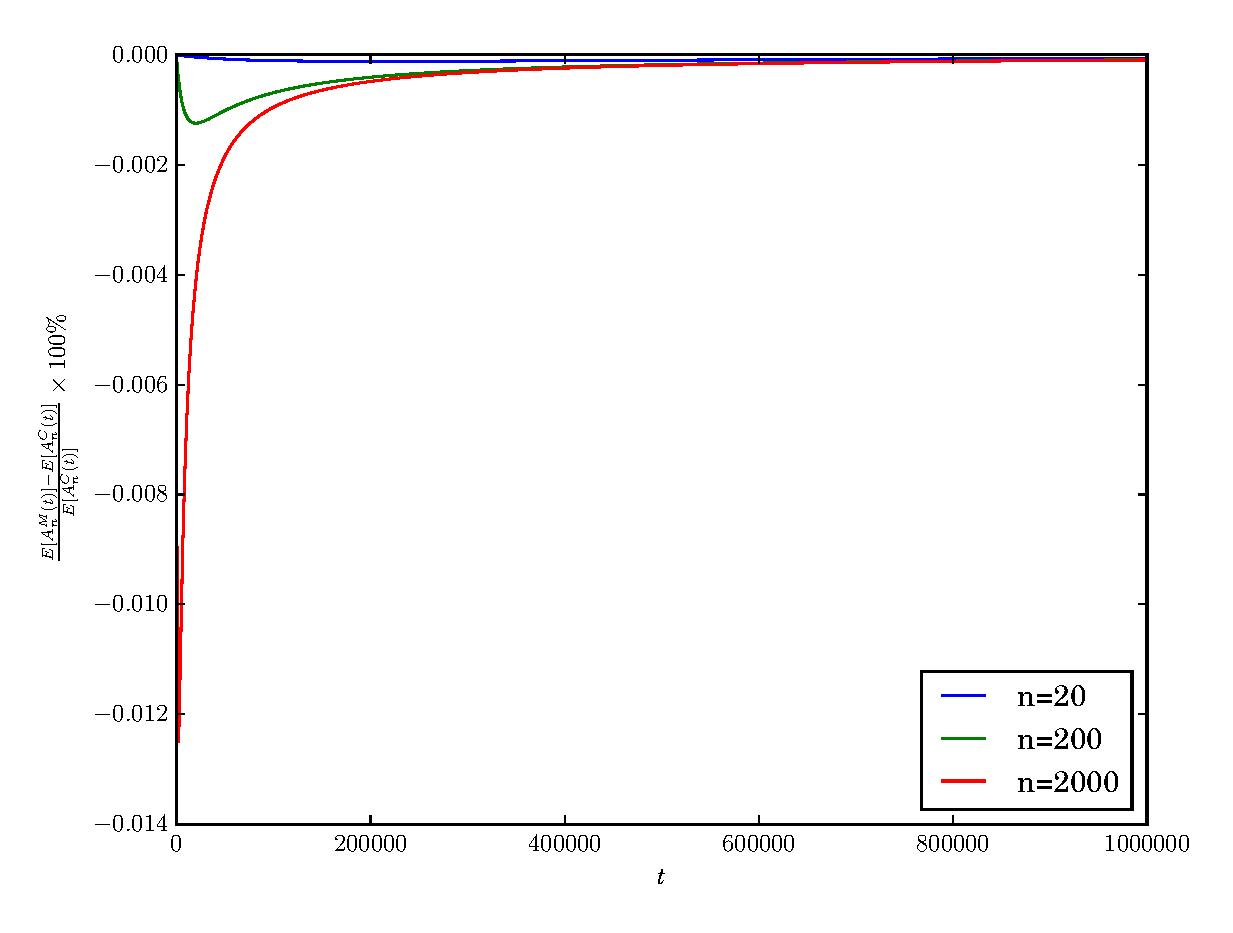
\includegraphics[scale=0.7]{../plots/moran_figure4}
		\end{subfigure}
		\caption{Plots of the percent difference in the NLFT under the Moran model compared to the Coalescent. The top panel is with a constant population size of $N=20000$ and the bottom is with a constant population size of $N=2000$. The general patterns are similar for a given fraction $(\frac{n}{N})$ that the sample size represents, although there tend to be larger maximum deviations in the case of smaller population size. This makes sense because in smaller population sizes we are farther from the diffusion limit under which the Coalescent is an appropriate approximation to the ancestral process.}
	\end{figure}

\end{center}


\end{document}



